% Options for packages loaded elsewhere
\PassOptionsToPackage{unicode}{hyperref}
\PassOptionsToPackage{hyphens}{url}
%
\documentclass[
]{book}
\usepackage{amsmath,amssymb}
\usepackage{iftex}
\ifPDFTeX
  \usepackage[T1]{fontenc}
  \usepackage[utf8]{inputenc}
  \usepackage{textcomp} % provide euro and other symbols
\else % if luatex or xetex
  \usepackage{unicode-math} % this also loads fontspec
  \defaultfontfeatures{Scale=MatchLowercase}
  \defaultfontfeatures[\rmfamily]{Ligatures=TeX,Scale=1}
\fi
\usepackage{lmodern}
\ifPDFTeX\else
  % xetex/luatex font selection
\fi
% Use upquote if available, for straight quotes in verbatim environments
\IfFileExists{upquote.sty}{\usepackage{upquote}}{}
\IfFileExists{microtype.sty}{% use microtype if available
  \usepackage[]{microtype}
  \UseMicrotypeSet[protrusion]{basicmath} % disable protrusion for tt fonts
}{}
\makeatletter
\@ifundefined{KOMAClassName}{% if non-KOMA class
  \IfFileExists{parskip.sty}{%
    \usepackage{parskip}
  }{% else
    \setlength{\parindent}{0pt}
    \setlength{\parskip}{6pt plus 2pt minus 1pt}}
}{% if KOMA class
  \KOMAoptions{parskip=half}}
\makeatother
\usepackage{xcolor}
\usepackage{color}
\usepackage{fancyvrb}
\newcommand{\VerbBar}{|}
\newcommand{\VERB}{\Verb[commandchars=\\\{\}]}
\DefineVerbatimEnvironment{Highlighting}{Verbatim}{commandchars=\\\{\}}
% Add ',fontsize=\small' for more characters per line
\usepackage{framed}
\definecolor{shadecolor}{RGB}{248,248,248}
\newenvironment{Shaded}{\begin{snugshade}}{\end{snugshade}}
\newcommand{\AlertTok}[1]{\textcolor[rgb]{0.94,0.16,0.16}{#1}}
\newcommand{\AnnotationTok}[1]{\textcolor[rgb]{0.56,0.35,0.01}{\textbf{\textit{#1}}}}
\newcommand{\AttributeTok}[1]{\textcolor[rgb]{0.13,0.29,0.53}{#1}}
\newcommand{\BaseNTok}[1]{\textcolor[rgb]{0.00,0.00,0.81}{#1}}
\newcommand{\BuiltInTok}[1]{#1}
\newcommand{\CharTok}[1]{\textcolor[rgb]{0.31,0.60,0.02}{#1}}
\newcommand{\CommentTok}[1]{\textcolor[rgb]{0.56,0.35,0.01}{\textit{#1}}}
\newcommand{\CommentVarTok}[1]{\textcolor[rgb]{0.56,0.35,0.01}{\textbf{\textit{#1}}}}
\newcommand{\ConstantTok}[1]{\textcolor[rgb]{0.56,0.35,0.01}{#1}}
\newcommand{\ControlFlowTok}[1]{\textcolor[rgb]{0.13,0.29,0.53}{\textbf{#1}}}
\newcommand{\DataTypeTok}[1]{\textcolor[rgb]{0.13,0.29,0.53}{#1}}
\newcommand{\DecValTok}[1]{\textcolor[rgb]{0.00,0.00,0.81}{#1}}
\newcommand{\DocumentationTok}[1]{\textcolor[rgb]{0.56,0.35,0.01}{\textbf{\textit{#1}}}}
\newcommand{\ErrorTok}[1]{\textcolor[rgb]{0.64,0.00,0.00}{\textbf{#1}}}
\newcommand{\ExtensionTok}[1]{#1}
\newcommand{\FloatTok}[1]{\textcolor[rgb]{0.00,0.00,0.81}{#1}}
\newcommand{\FunctionTok}[1]{\textcolor[rgb]{0.13,0.29,0.53}{\textbf{#1}}}
\newcommand{\ImportTok}[1]{#1}
\newcommand{\InformationTok}[1]{\textcolor[rgb]{0.56,0.35,0.01}{\textbf{\textit{#1}}}}
\newcommand{\KeywordTok}[1]{\textcolor[rgb]{0.13,0.29,0.53}{\textbf{#1}}}
\newcommand{\NormalTok}[1]{#1}
\newcommand{\OperatorTok}[1]{\textcolor[rgb]{0.81,0.36,0.00}{\textbf{#1}}}
\newcommand{\OtherTok}[1]{\textcolor[rgb]{0.56,0.35,0.01}{#1}}
\newcommand{\PreprocessorTok}[1]{\textcolor[rgb]{0.56,0.35,0.01}{\textit{#1}}}
\newcommand{\RegionMarkerTok}[1]{#1}
\newcommand{\SpecialCharTok}[1]{\textcolor[rgb]{0.81,0.36,0.00}{\textbf{#1}}}
\newcommand{\SpecialStringTok}[1]{\textcolor[rgb]{0.31,0.60,0.02}{#1}}
\newcommand{\StringTok}[1]{\textcolor[rgb]{0.31,0.60,0.02}{#1}}
\newcommand{\VariableTok}[1]{\textcolor[rgb]{0.00,0.00,0.00}{#1}}
\newcommand{\VerbatimStringTok}[1]{\textcolor[rgb]{0.31,0.60,0.02}{#1}}
\newcommand{\WarningTok}[1]{\textcolor[rgb]{0.56,0.35,0.01}{\textbf{\textit{#1}}}}
\usepackage{longtable,booktabs,array}
\usepackage{calc} % for calculating minipage widths
% Correct order of tables after \paragraph or \subparagraph
\usepackage{etoolbox}
\makeatletter
\patchcmd\longtable{\par}{\if@noskipsec\mbox{}\fi\par}{}{}
\makeatother
% Allow footnotes in longtable head/foot
\IfFileExists{footnotehyper.sty}{\usepackage{footnotehyper}}{\usepackage{footnote}}
\makesavenoteenv{longtable}
\usepackage{graphicx}
\makeatletter
\def\maxwidth{\ifdim\Gin@nat@width>\linewidth\linewidth\else\Gin@nat@width\fi}
\def\maxheight{\ifdim\Gin@nat@height>\textheight\textheight\else\Gin@nat@height\fi}
\makeatother
% Scale images if necessary, so that they will not overflow the page
% margins by default, and it is still possible to overwrite the defaults
% using explicit options in \includegraphics[width, height, ...]{}
\setkeys{Gin}{width=\maxwidth,height=\maxheight,keepaspectratio}
% Set default figure placement to htbp
\makeatletter
\def\fps@figure{htbp}
\makeatother
\setlength{\emergencystretch}{3em} % prevent overfull lines
\providecommand{\tightlist}{%
  \setlength{\itemsep}{0pt}\setlength{\parskip}{0pt}}
\setcounter{secnumdepth}{5}
\usepackage{booktabs}
\ifLuaTeX
  \usepackage{selnolig}  % disable illegal ligatures
\fi
\usepackage[]{natbib}
\bibliographystyle{plainnat}
\usepackage{bookmark}
\IfFileExists{xurl.sty}{\usepackage{xurl}}{} % add URL line breaks if available
\urlstyle{same}
\hypersetup{
  pdftitle={ADS - Engenharia de Software 2025 - Anotações de aula},
  pdfauthor={Professor Miguel Suez Xve Penteado},
  hidelinks,
  pdfcreator={LaTeX via pandoc}}

\title{ADS - Engenharia de Software 2025 - Anotações de aula}
\author{Professor Miguel Suez Xve Penteado}
\date{2025-02-25}

\begin{document}
\maketitle

{
\setcounter{tocdepth}{1}
\tableofcontents
}
\chapter*{Sobre estas anotações}\label{sobre-estas-anotauxe7uxf5es}
\addcontentsline{toc}{chapter}{Sobre estas anotações}

Estas anotações são apenas lembretes das aulas expostas em sala, durante a disciplina de ENGENHARIA DE SOFTWARE.

\section{ACESSO AO GITBOOK CELULAR}\label{acesso-ao-gitbook-celular}

\section{\texorpdfstring{\url{https://miguel7penteado.github.io/ADS-EngenhariaSoftware2025}}{https://miguel7penteado.github.io/ADS-EngenhariaSoftware2025}}\label{httpsmiguel7penteado.github.ioads-engenhariasoftware2025}


\includegraphics{images/clipboard-3692082511.png}

\section{APP EPUB ANDROID}\label{app-epub-android}

\section{\texorpdfstring{\textbf{Moon+ Reader}}{Moon+ Reader}}\label{moon-reader}


\includegraphics{images/qrcode/leitor_epub/MoonReaderPlus.jpg}

\chapter{Livros Texto da Disciplina}\label{livros-texto-da-disciplina}

\subsubsection{``Engenharia de Software'' do autor ``Roger S Pressman''}\label{engenharia-de-software-do-autor-roger-s-pressman}

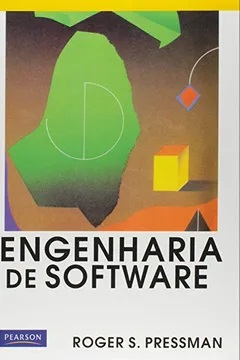
\includegraphics{images/livros/engenharia_software_pressman.jpg}

\begin{longtable}[]{@{}
  >{\raggedright\arraybackslash}p{(\columnwidth - 2\tabcolsep) * \real{0.5000}}
  >{\raggedright\arraybackslash}p{(\columnwidth - 2\tabcolsep) * \real{0.5000}}@{}}
\toprule\noalign{}
\endhead
\bottomrule\noalign{}
\endlastfoot
\textbf{Autor(es)} & \href{https://www.indicalivros.com/autores?q=Roger\%20S.\%20Pressman}{Roger S. Pressman} \\
\textbf{Editora} & Pearson \\
\textbf{Idioma} & Português \\
\textbf{ISBN} & 8534602379 9788534602372 \\
\textbf{Formato} & Capa comum \\
\textbf{Páginas} & 1056 \\
\textbf{Código Biblioteca} & \\
\end{longtable}

\subsubsection{``Engenharia de Software'' do autor ``Ian Sommerville''}\label{engenharia-de-software-do-autor-ian-sommerville}

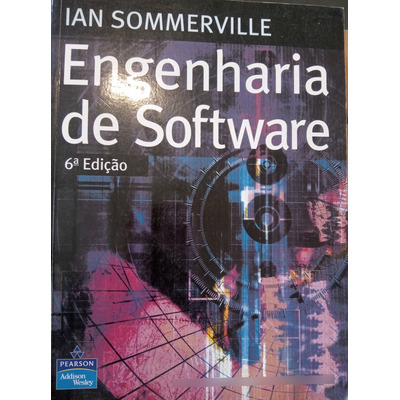
\includegraphics{images/livros/engenharia_software_sommerville.jpg}

\begin{longtable}[]{@{}ll@{}}
\toprule\noalign{}
\endhead
\bottomrule\noalign{}
\endlastfoot
\textbf{Autor(es)} & Ian SommerVille \\
\textbf{Editora} & Pearson \\
\textbf{Idioma} & Português \\
\textbf{ISBN} & 9788588639072 \\
\textbf{Formato} & Capa comum \\
\textbf{Páginas} & 768 \\
\textbf{Código Biblioteca} & \\
\end{longtable}

Calendário das aulas

\paragraph{FEVEREIRO 2025}\label{fevereiro-2025}

\begin{longtable}[]{@{}lll@{}}
\toprule\noalign{}
\endhead
\bottomrule\noalign{}
\endlastfoot
Data & Dia da semana & Aulas \\
4 de fevereiro & Terça-feira & \\
11 de fevereiro & Terça-feira & \\
18 de fevereiro & Terça-feira & Aula Inaugural \\
25 de fevereiro & Terça-feira & \\
\end{longtable}

\paragraph{MARÇO 2025}\label{maruxe7o-2025}

\begin{longtable}[]{@{}lll@{}}
\toprule\noalign{}
\endhead
\bottomrule\noalign{}
\endlastfoot
Data & Dia da semana & Aulas \\
4 de março & Terça-feira & \\
11 de março & Terça-feira & \\
18 de março & Terça-feira & \\
25 de março & Terça-feira & \\
\end{longtable}

\paragraph{ABRIL DE 2025}\label{abril-de-2025}

\begin{longtable}[]{@{}lll@{}}
\toprule\noalign{}
\endhead
\bottomrule\noalign{}
\endlastfoot
Data & Dia da semana & Aulas \\
1 de abril & Terça-feira & \\
8 de abril & Terça-feira & \\
15 de abril & Terça-feira & \\
22 de abril & Terça-feira & \\
29 de abril & Terça-feira & \\
\end{longtable}

\paragraph{MAIO DE 2025}\label{maio-de-2025}

\begin{longtable}[]{@{}lll@{}}
\toprule\noalign{}
\endhead
\bottomrule\noalign{}
\endlastfoot
Data & Dia da semana & Aulas \\
6 de maio & Terça-feira & \\
13 de maio & Terça-feira & \\
20 de maio & Terça-feira & \\
27 de maio & Terça-feira & \\
\end{longtable}

\paragraph{JUNHO DE 2025}\label{junho-de-2025}

\begin{longtable}[]{@{}lll@{}}
\toprule\noalign{}
\endhead
\bottomrule\noalign{}
\endlastfoot
Data & Dia da semana & Aulas \\
3 de junho & Terça-feira & \\
10 de junho & Terça-feira & \\
17 de junho & Terça-feira & \\
24 de junho & Terça-feira & \\
\end{longtable}

\begin{Shaded}
\begin{Highlighting}[]
\NormalTok{bookdown}\SpecialCharTok{::}\FunctionTok{render\_book}\NormalTok{()}
\end{Highlighting}
\end{Shaded}

\chapter*{INTRODUÇÃO A DISCIPLINA DE ENGENHARIA DE SOFTWARE}\label{introduuxe7uxe3o-a-disciplina-de-engenharia-de-software}
\addcontentsline{toc}{chapter}{INTRODUÇÃO A DISCIPLINA DE ENGENHARIA DE SOFTWARE}

Do que trata esta disciplina e o que quer dizer o termo que dá nome a ela ?

\section{O que é ENGENHARIA DE SOFTWARE}\label{o-que-uxe9-engenharia-de-software}

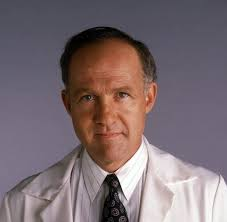
\includegraphics[width=0.95833in,height=\textheight]{images/pressman.jpg}

\begin{quote}
\textbf{Engenharia de Software}~\emph{é o processo de desenvolvimento de programas de computador, estruturas de dados e documentos.} (\textbf{\emph{Roger S. Pressman}})
\end{quote}

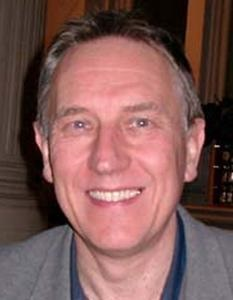
\includegraphics[width=1.0625in,height=\textheight]{images/sommerville.jpg}

\begin{quote}
\textbf{Engenharia de Software} \emph{é uma disciplina de engenharia que se preocupa com todo o processo de produção de software. Isso inclui desde a especificação do sistema até a sua manutenção.} (\textbf{Ian Sommerville})
\end{quote}

É atribuído a \textbf{Margaret Hamilton,} desenvolvedora do programa de navegação da APOLLO 11 a criação do termo ENGENHARIA DE SOFTWARE.

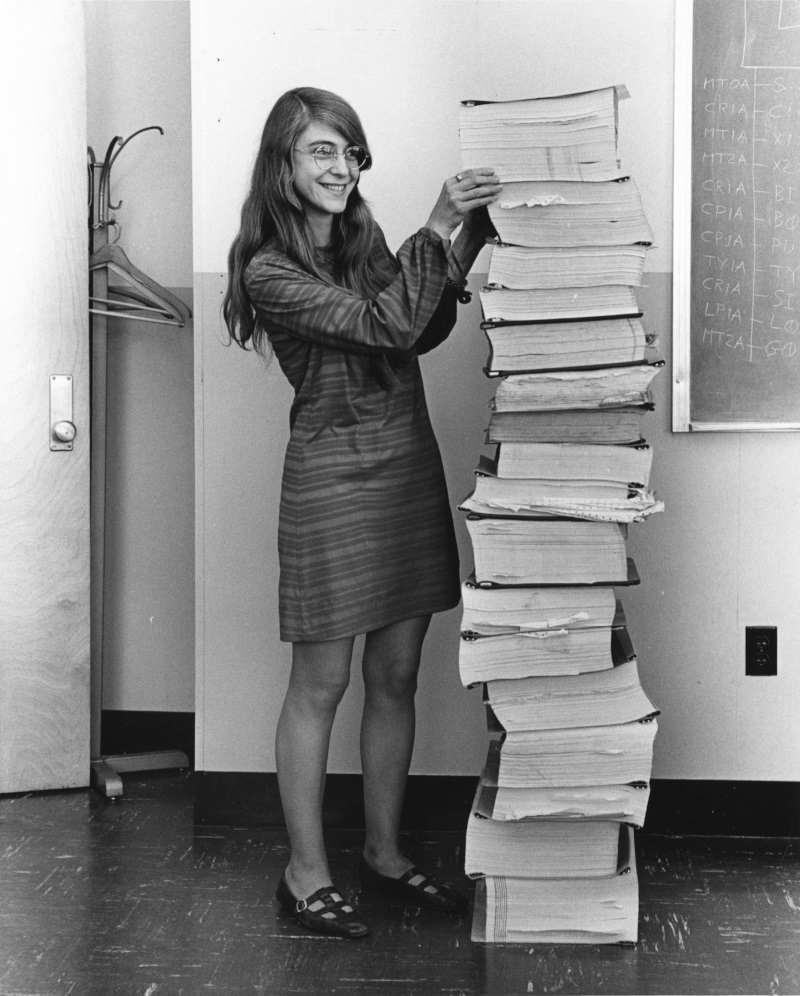
\includegraphics[width=0.5\textwidth,height=\textheight]{images/Margaret_Hamilton.jpg}

\chapter{QUALIDADE DE SOFTWARE}\label{qualidade-de-software}

\section{COMPLIANCE}\label{compliance}

Para que uma organização consiga fechar contrados de venda ou fornecimento com outra organização, especialmente quando o valor do contrato de venda ou prestação é muito alto, há um processo de checagem de COMPLIANCE:

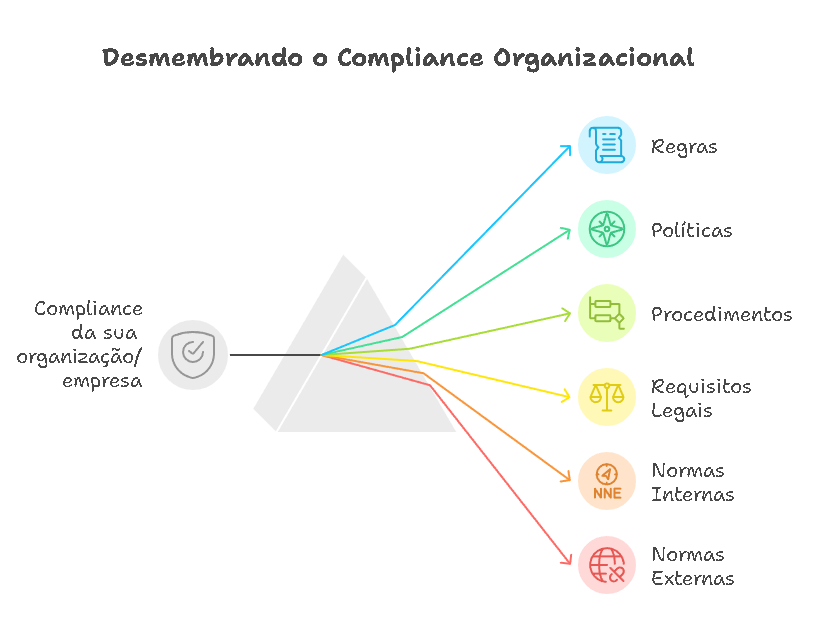
\includegraphics{images/qualidade-geral/compliance.png}

\section{QUALIDADE}\label{qualidade}

O que é Qualidade ? (Definição ISO 9000)

\begin{quote}
Qualidade é definida como o grau em que um conjunto de características inerentes de um objeto satisfaz requisitos onde: \textbf{Características inerentes} São propriedades que fazem parte do objeto, onde:

\begin{itemize}
\item
  \textbf{Requisitos}: São as necessidades ou expectativas declaradas, geralmente implícitas ou obrigatórias;
\item
  \textbf{objeto} pode ser representado por um produto, serviço, processo, organização, sistema ou pessoa;
\end{itemize}
\end{quote}

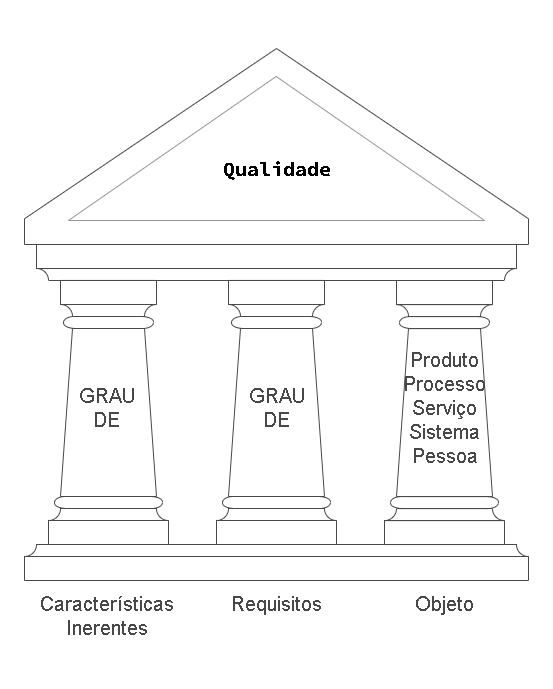
\includegraphics{images/qualidade-geral/Qualidade.png}

\subsection{QUALIDADE APLICADA A PRODUTO}\label{qualidade-aplicada-a-produto}

O CONTROLE DE QUALIDADE do PRODUTO concentra-se em aperfeiçoar:

\begin{itemize}
\item
  as \textbf{características} e
\item
  o \textbf{desempenho} do produto em si,
\end{itemize}

visando atender às necessidades e expectativas dos clientes.

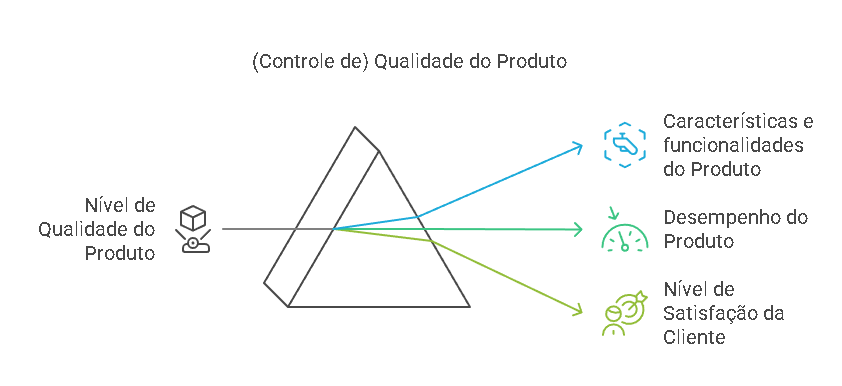
\includegraphics{images/qualidade-geral/Qualidade_do_Produto.png}

\subsection{QUALIDADE APLICADA A PROCESSO}\label{qualidade-aplicada-a-processo}

O CONTROLE DE QUALIDADE DE PROCESSO concentra-se em aperfeiçoar

\begin{itemize}
\item
  as \textbf{atividades} e
\item
  melhor \textbf{aplicação dos recursos}
\end{itemize}

utilizados para criar o produto, visando garantir a consistência e a eficácia da produção.

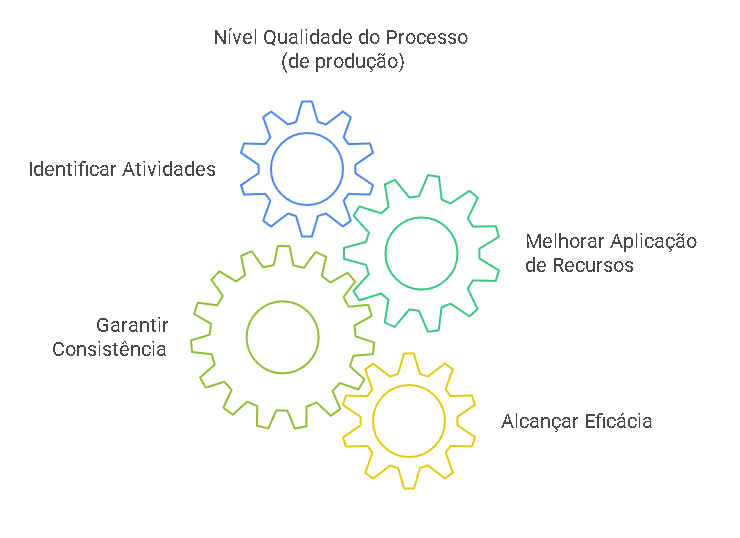
\includegraphics{images/qualidade-geral/Qualidade_do_Processo.png}

\subsection{CASO MACDONALDS - Qualidade de Produto e Processo}\label{caso-macdonalds---qualidade-de-produto-e-processo}

O filme ``Fome de Poder'' (``The Founder'', no original) narra a história real da ascensão da rede McDonald's, desde sua origem como uma pequena hamburgueria na Califórnia até se tornar um império global do fast-food.

\begin{itemize}
\tightlist
\item
  Reconhecimento da \textbf{qualidade do produto} - hamburguers McDonalds
\end{itemize}

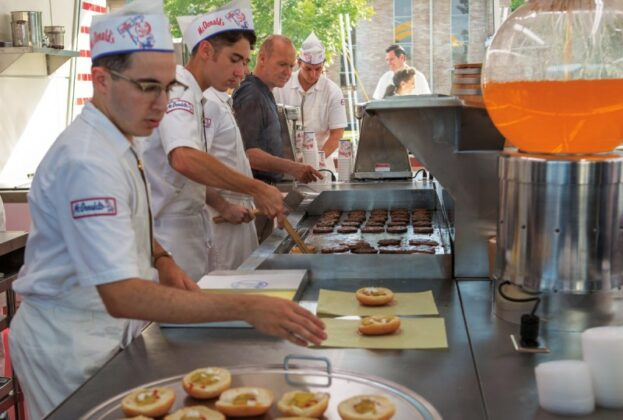
\includegraphics{images/mac-donalds/cozinha-mac.jpg}

Reconhecimento da \textbf{Qualidade do Processo} de fabricação do Produto

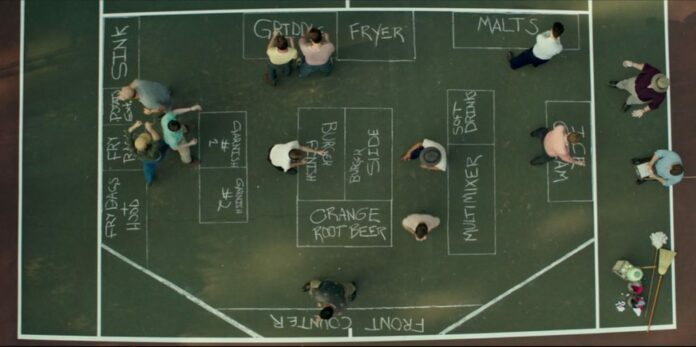
\includegraphics{images/mac-donalds/modelo-mac.jpg}

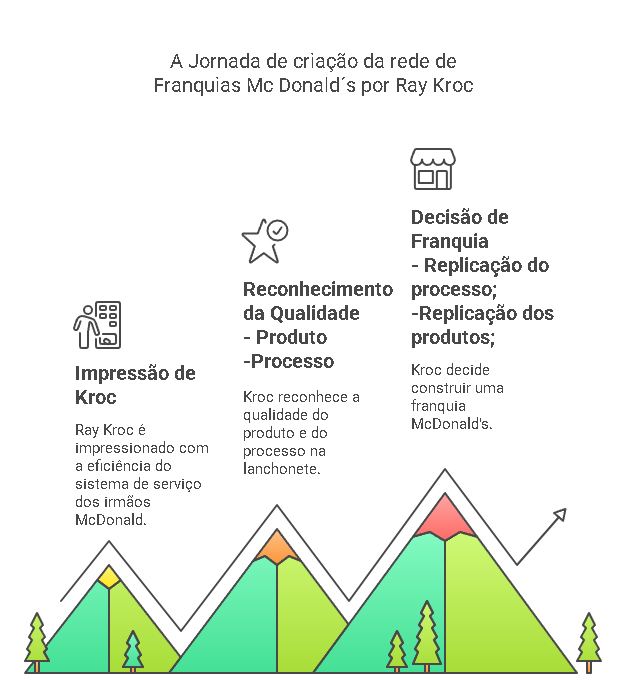
\includegraphics{images/qualidade-geral/MacDonalds1.png}

\begin{itemize}
\tightlist
\item
  Reconhecimento da Capacidade de Franquia (Replicação):
\end{itemize}

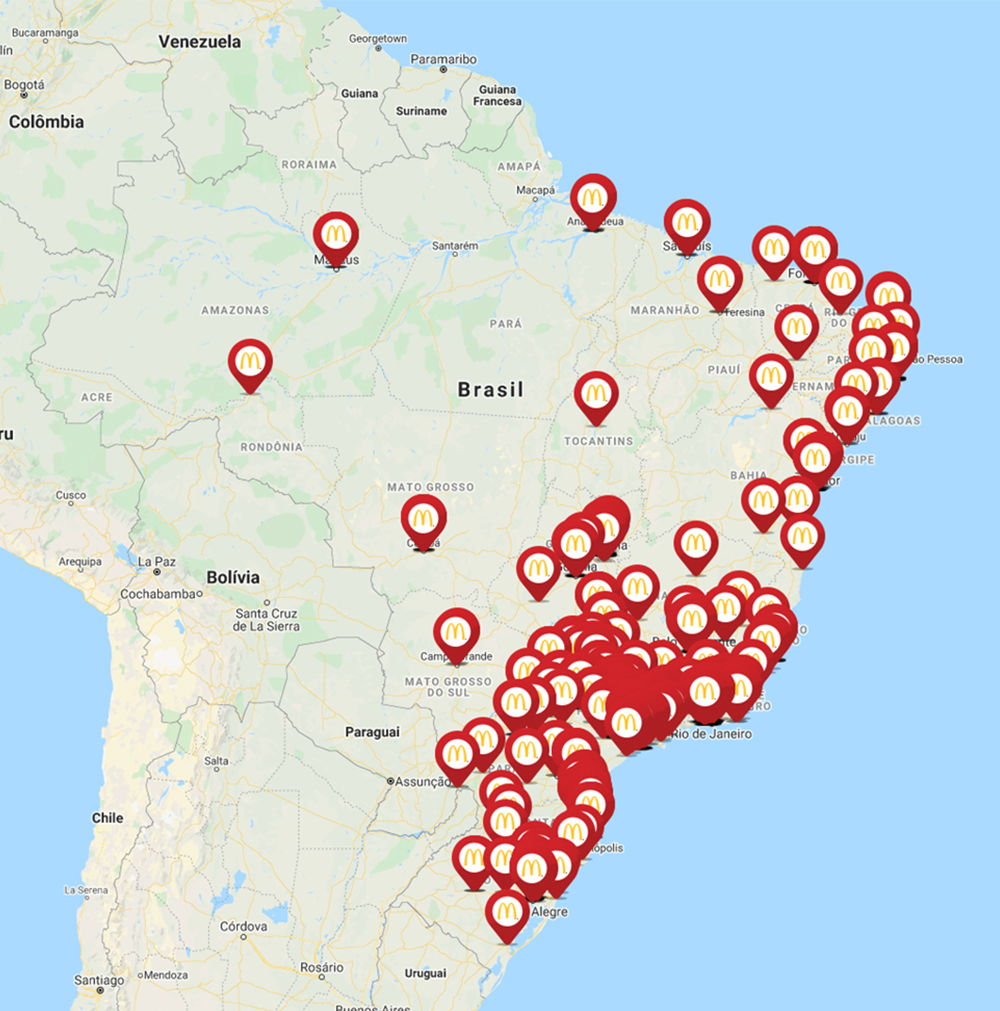
\includegraphics[width=4.23958in,height=\textheight]{images/mac-donalds/Franquias.jpg}

\subsection{QUALIDADE NAS ORGANIZAÇÕES}\label{qualidade-nas-organizauxe7uxf5es}

\subsection{Família ISO 9000}\label{famuxedlia-iso-9000}

\textbf{A NBR ISO 9000} é um conjunto de normas técnicas que estabelecem diretrizes e padrões para a criação de um \textbf{Sistema de Gestão da Qualidade (SGQ)}.

O sistema SGQ (um si que pode ou não ser um pacote de software) deve mapear

\begin{longtable}[]{@{}
  >{\centering\arraybackslash}p{(\columnwidth - 8\tabcolsep) * \real{0.2000}}
  >{\centering\arraybackslash}p{(\columnwidth - 8\tabcolsep) * \real{0.2000}}
  >{\centering\arraybackslash}p{(\columnwidth - 8\tabcolsep) * \real{0.2000}}
  >{\centering\arraybackslash}p{(\columnwidth - 8\tabcolsep) * \real{0.2000}}
  >{\centering\arraybackslash}p{(\columnwidth - 8\tabcolsep) * \real{0.2000}}@{}}
\toprule\noalign{}
\endhead
\bottomrule\noalign{}
\endlastfoot
Áreas mapeadas por um sistema SGQ & PROCESSOS & POLÍTICAS & PROCEDIMENTOS & RESPONSABILIDADES \\
\end{longtable}

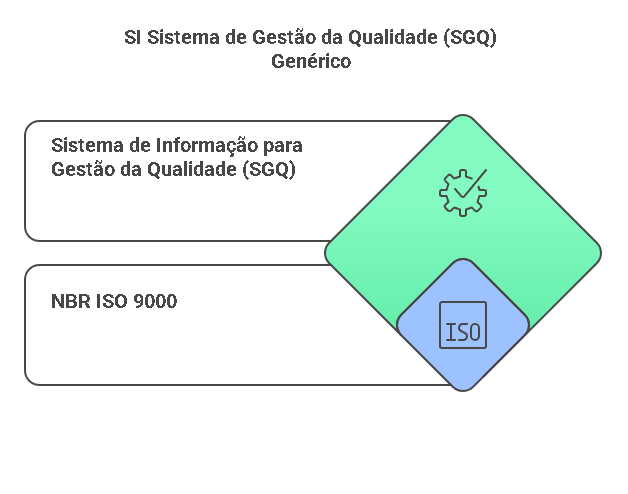
\includegraphics[width=5.71875in,height=\textheight]{images/qualidade-geral/ISO-9000-SGQ.png}

\subsection{Família ISO 14000}\label{famuxedlia-iso-14000}

\textbf{A NBR ISO 14000} é um conjunto de normas técnicas que tratam de GESTÃO AMBIENTAL nas organizações. Estabelecem normas e diretrizes para criar \textbf{(SI) Sistemas de Gestão Ambiental (SGA)}:

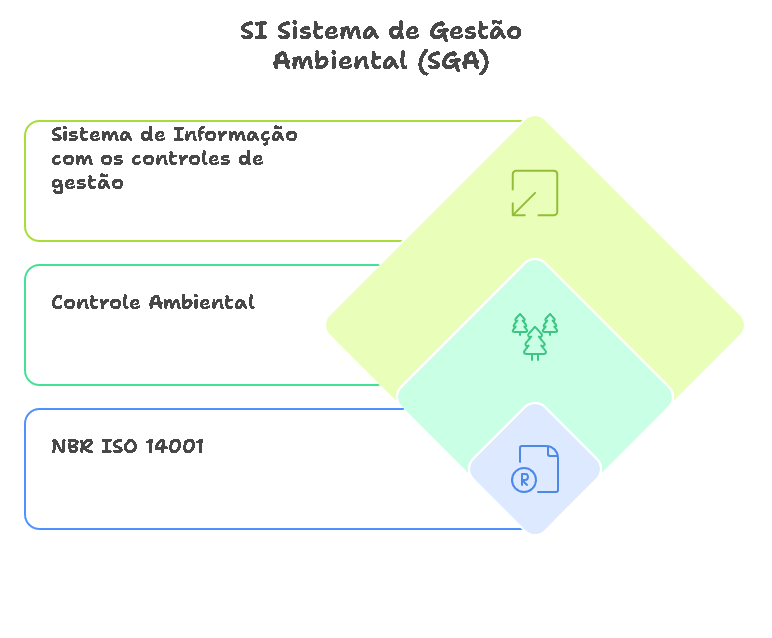
\includegraphics{images/qualidade-geral/ISO-14000-SGQ.png}

\subsection{Família ISO 27000}\label{famuxedlia-iso-27000}

\textbf{NBR ISO 27000}, trata de normas para \textbf{gestão segurança da Informação.} Fornecem um framework para a gestão da segurança da informação em organizações.

Especifica os requisitos para um para a criação de um(SI) Sistema de Gestão de Segurança da Informação (SGSI).

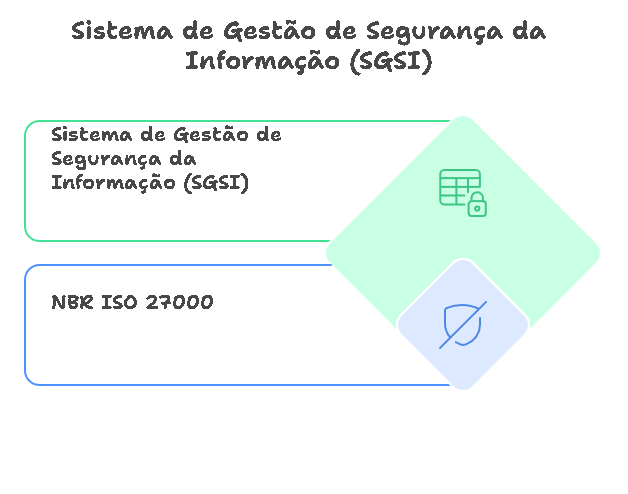
\includegraphics{images/qualidade-geral/ISO-27000-SGSI.png}

\subsection{Segmentos das Organizações e Adoção das normas de Qualidade}\label{segmentos-das-organizauxe7uxf5es-e-adouxe7uxe3o-das-normas-de-qualidade}

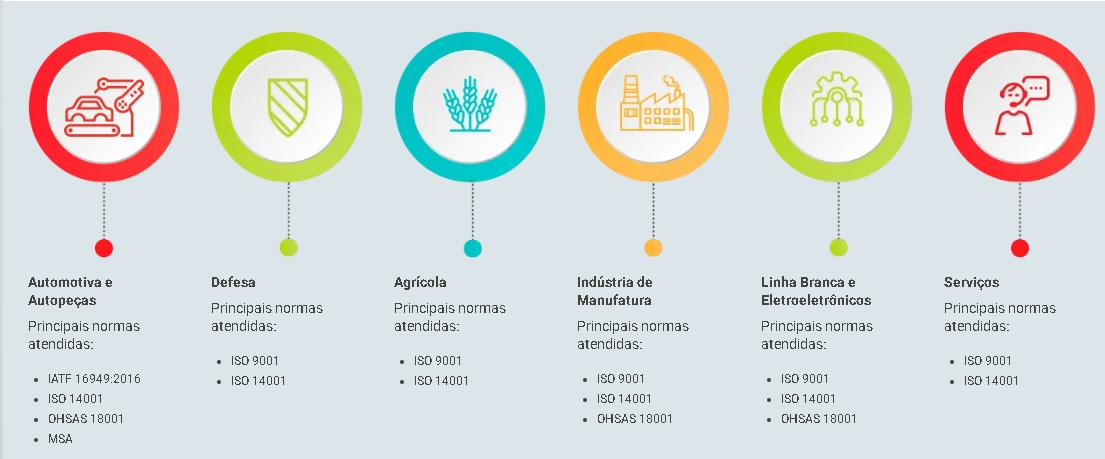
\includegraphics{images/qualidade-geral/segmentos.jpg}

\subsection{QUALIDADE NA ENGENHARIA DE SOFTWARE}\label{qualidade-na-engenharia-de-software}

A qualidade de software não define S.I.s

\subsection{Família NBR ISO 9126}\label{famuxedlia-nbr-iso-9126}

Focava na qualidade do produto de software, definindo um conjunto de parâmetros para padronizar a avaliação dessa qualidade. Ela se enquadrava no modelo de qualidade das normas da família 9000.

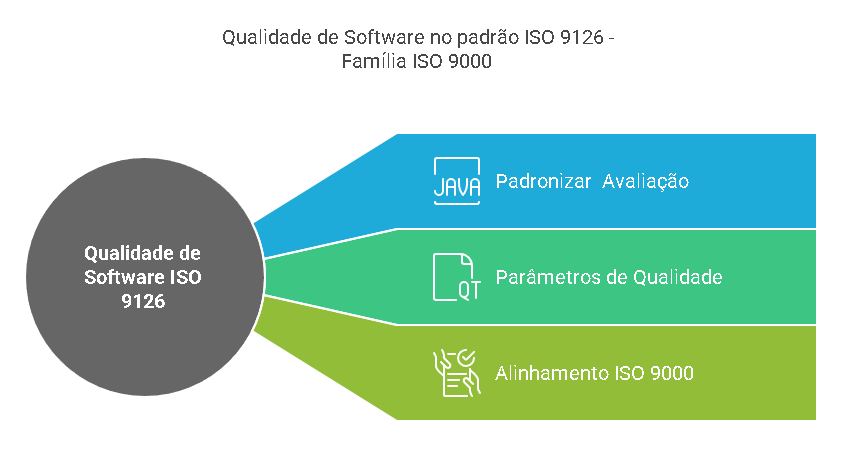
\includegraphics{images/qualidade-geral/ISO-9126-SGSI.png}

\subsection{Família NBR ISO 12207}\label{famuxedlia-nbr-iso-12207}

A norma ISO 12207 define um conjunto de processos para o ciclo de vida do software. Seu principal foco é estabelecer um framework padronizado para o desenvolvimento, manutenção e descarte de software, visando garantir a qualidade e a eficiência desses processos.

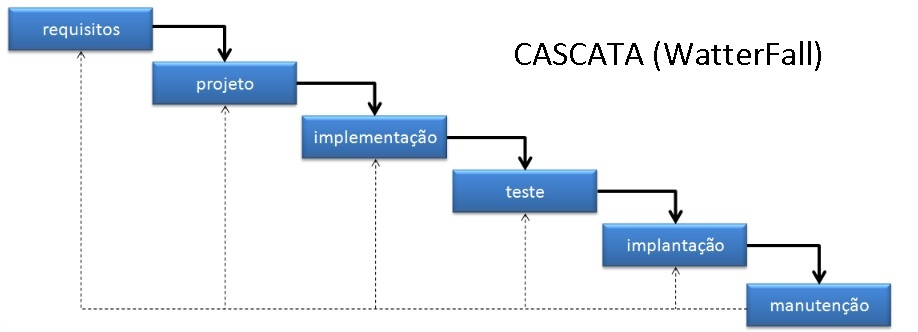
\includegraphics{images/modelos_processos_software/Cascata.jpg}

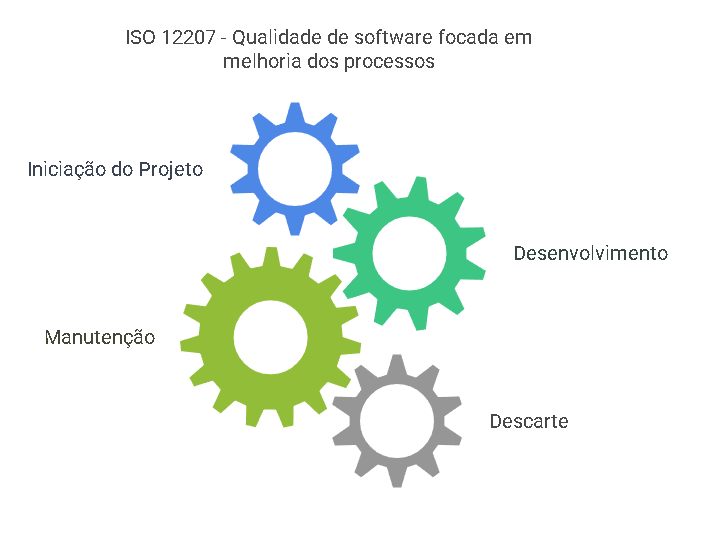
\includegraphics{images/qualidade-geral/ISO-12207-processos.png}

\subsection{Família NBR ISO 25000}\label{famuxedlia-nbr-iso-25000}

\textbf{A NBR ISO 25000}, também conhecida como SQuaRE (Software Product Quality Requirements and Evaluation - Requisitos e Avaliação da Qualidade de Produtos de Software), é uma série de normas internacionais que fornecem um subconjunto de normas para a avaliação da qualidade de produtos de software. Este subconjunto é formado pelas normas \textbf{ISO/IEC 25000} , \textbf{ISO/IEC 25010}, \textbf{ISO/IEC 25020}, \textbf{ISO/IEC 25030} e \textbf{ISO/IEC 25040}.

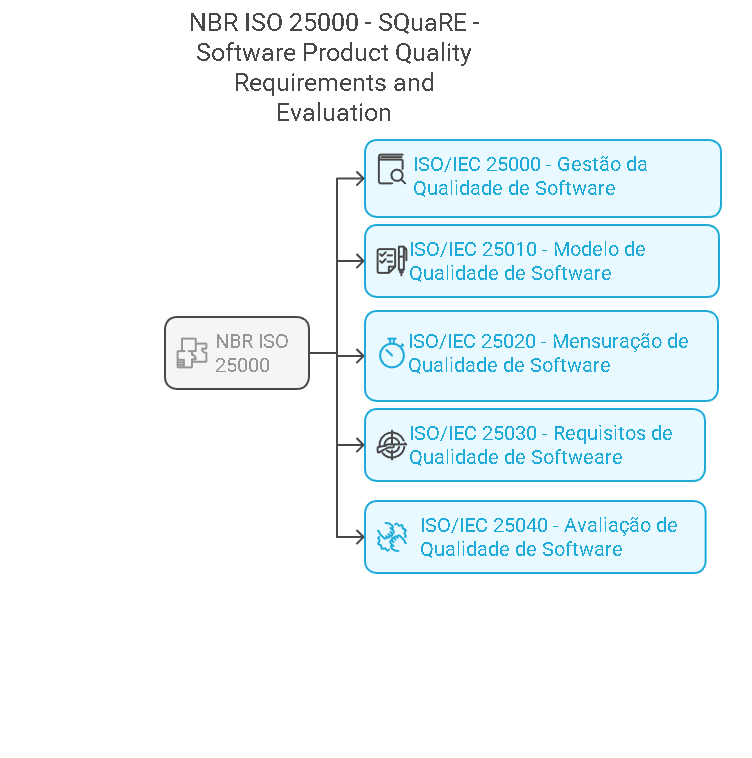
\includegraphics{images/qualidade-geral/ISO-25000-SQuaRE.png}

\chapter{MODELAGEM DE SOFTWARE}\label{modelagem-de-software}

Coming soon

\chapter{GESTÃO DE QUALIDADE DE SOFTWARE}\label{gestuxe3o-de-qualidade-de-software}

Coming soon

\chapter{GERÊNCIA DE PROJETOS}\label{geruxeancia-de-projetos}

Coming soon

\chapter{Sharing your book}\label{sharing-your-book}

\section{Publishing}\label{publishing}

HTML books can be published online, see: \url{https://bookdown.org/yihui/bookdown/publishing.html}

\section{404 pages}\label{pages}

By default, users will be directed to a 404 page if they try to access a webpage that cannot be found. If you'd like to customize your 404 page instead of using the default, you may add either a \texttt{\_404.Rmd} or \texttt{\_404.md} file to your project root and use code and/or Markdown syntax.

\section{Metadata for sharing}\label{metadata-for-sharing}

Bookdown HTML books will provide HTML metadata for social sharing on platforms like Twitter, Facebook, and LinkedIn, using information you provide in the \texttt{index.Rmd} YAML. To setup, set the \texttt{url} for your book and the path to your \texttt{cover-image} file. Your book's \texttt{title} and \texttt{description} are also used.

This \texttt{gitbook} uses the same social sharing data across all chapters in your book- all links shared will look the same.

Specify your book's source repository on GitHub using the \texttt{edit} key under the configuration options in the \texttt{\_output.yml} file, which allows users to suggest an edit by linking to a chapter's source file.

Read more about the features of this output format here:

\url{https://pkgs.rstudio.com/bookdown/reference/gitbook.html}

Or use:

\begin{Shaded}
\begin{Highlighting}[]
\NormalTok{?bookdown}\SpecialCharTok{::}\NormalTok{gitbook}
\end{Highlighting}
\end{Shaded}


  \bibliography{book.bib,packages.bib}

\end{document}
